% Template for ICASSP-2021 paper; to be used with:
%          spconf.sty  - ICASSP/ICIP LaTeX style file, and
%          IEEEbib.bst - IEEE bibliography style file.
% --------------------------------------------------------------------------
\documentclass{article}
\usepackage{spconf,amsmath,graphicx,xcolor}
\usepackage{hyperref}
\usepackage{bbold}
\usepackage{amsfonts}
\usepackage[ruled,vlined]{algorithm2e}
\usepackage{booktabs}
\usepackage{graphicx}
\graphicspath{ {./images/}  }

\title{Last layer state space model}
%
% Single address.
% ---------------
\name{Max Cohen$^{\star \dagger}$ \qquad Sylvain Le Corff$^{\star}$ \qquad Maurice Charbit$^{\dagger}$ \qquad Gilles Nozière$^{\dagger}$}
\address{
	$^{\star}$Telecom SudParis\\
	$^{\dagger}$Oze Energies
}
%
% For example:
% ------------
%\address{School\\
%	Department\\
%	Address}
%
% Two addresses (uncomment and modify for two-address case).
% ----------------------------------------------------------
%\twoauthors
%  {A. Author-one, B. Author-two\sthanks{Thanks to XYZ agency for funding.}}
%	{School A-B\\
%	Department A-B\\
%	Address A-B}
%  {C. Author-three, D. Author-four\sthanks{The fourth author performed the work
%	while at ...}}
%	{School C-D\\
%	Department C-D\\
%	Address C-D}
%

\begin{document}
\maketitle

\begin{abstract}
	As sequential neural architectures become deeper and more complex, estimating the uncertainty of their predictions is ever so challenging.
	Efforts in quantifying uncertainty often rely on specific training procedures, and bear additional computational costs due to the dimensionality of such models.
	In this paper, we demonstrate how uncertainty can be estimated on top of an existing and trained neural network, combining a state space-based last  layer and  Sequential Monte Carlo methods. This approach allows to separate representation learning and uncertainty quantification. We apply our proposed methodology for the estimation of air quality in office buildings, through the hourly prediction of \ensuremath{\mathrm{CO_2}} and humidity levels.
	Our model accounts for the noisy data structure, due to unknown or unavailable variables (occupancy of the building, manual ventilation, etc.), and is able to provide confidence intervals on predictions.
\end{abstract}

\begin{keywords}
	Recurrent neural networks, Uncertainty quantification, Sequential Monte Carlo.
\end{keywords}

\section{Introduction}
\label{sec:intro}
% We believe a deeper understanding of \ensuremath{\mathrm{CO_2}} variations can assist in regulating and reducing HVAC consumption, while improving well being.

Recurrent Neural Networks (RNN) were first introduced as an efficient and convenient architecture to address short time dependencies problems \cite{Mozer1989AFB}.
They have been consistently improved to develop longer term memory, and optimize their implementations \cite{Bengio1994LearningLD,Hochreiter1997LongSM,Cho2014LearningPR}.
Current deep learning framework allows stacking arbitrary high number of recurrent layers, whose parameters are estimated by gradient descent through an automated differentiation procedure.

These recurrent architectures are able to approximate complex nonlinear time series, but suffer from overconfidence when evaluated outside of their training observations. Bayesian statistics aim at mitigating this drawback by providing uncertainty estimation \cite{Hinton1995BayesianLF,MacKay1992}.

Several architectures inspired by variational inference emerged by considering latent states as random variables and approximating the posterior.
The authors of \cite{Chung2015NIPS} built on a traditional RNN architecture by modelling temporal dependencies between these latent random states.
Results presented in \cite{Fortunato2017bayesian} yield improved performances when considering local gradient information for computing the posterior.
Similarly, introducing random variables directly into a neural network's weights can mitigate overconfidence, as demonstrated by the authors of \cite{Hinton1993}.
In \cite{Blundell2015}, weights are considered as distributions instead of vector values, allowing the network to make more reasonable predictions about unseen data.

Variational methods display encouraging results for modelling uncertainty in existing models, but require significant alteration of the model, as well as it's training mechanism.
In contrast, Monte Carlo Dropout (MC Dropout) methods offer to capture uncertainty by adding a single non parametric Dropout layer during both training and evaluation tasks, producing variable predictions from a single trained model, see \cite{Gal2016}.
These results were later extended to recurrent architectures in \cite{Gal2016NIPS}.
In the following years, MC Dropout methods have been applied in many industrial fields, such as anomaly detection (\cite{Zhu2017DeepAC}), flight delay prediction (\cite{Vandal2018}) or molecular simulations (\cite{Wen2020UncertaintyQI}).
Alternatively, ensemble methods consists in training distinct networks to obtain a combined prediction, as shown in \cite{Pearce2018}.
However, these frequentist approaches fail to guarantee proper calibration of the model, as highlighted by \cite{ashukha2020pitfalls}, and suffer various limitations, see \cite{Fong2020}.

In an effort to provide an alternative strategy with limited computation overhead, \cite{Brosse2020OnLA} suggests splitting training in two stages: representation learning and uncertainty estimation.
Their experiments indicate that the latter should be limited to the last layers of the model, as introducing randomness in the entire network increases complexity without offering much better results.

However, the benchmarked methods for uncertainty estimation cannot be applied in a time series context, as latent states are dependant.
Instead, we explore Sequential Monte Carlo methods, which were already successfully combined with recurrent neural network to tackle variable sequential problems, see \cite{Ma2020}.
We turn to \cite{Martin2020TheMC} for an example using more complex neural architectures, such as Transformer.
Particle filters have also proven reliable in other fields, such as presented in \cite{Liu2020LSTMPF} for object tracking.

In this paper, we introduce a new method for uncertainty estimation combining high expressivity, quality uncertainty estimations and ease of training.
Our proposed architecture is composed of an arbitrary sequential model, followed by a decoupled state space model layer.
The former can be fitted through a traditional gradient descent iteration, while the latter is trained using Sequential Monte Carlo methods.
Our uncertainty estimation layer can thus be built on top of an existing, already trained model. The model is presented in Section~\ref{sec:decoupling} and numerical experiments are displayed in Section~\ref{sec:exp}.

\section{Last layer decoupling}
\label{sec:decoupling}

\subsection{Proposed model}%
\label{sub:proposed_architecture}

Our proposed model can be decomposed into two decoupled blocks.
An input model $h_\varphi$ is responsible for extracting relevant features from the input time series. Then, the final hidden states of this network are fed to a Sequential Monte Carlo Layer (SMCL), based on a plain RNN, to design a generative model and allow uncertainty estimation.

In the following, for any sequence $(a_m,\ldots, a_n)$ with $n\geq m$, we use the short-hand notation $a_{m:n} = (a_m,\ldots, a_n)$. Let $T\ge 1$ be a given time horizon. We consider the regression task associated with observations $Y_{1:T}$ and inputs $U_{1:T}$, and denote by $X_{1:T}$ the hidden states of the model. For all $t\geq 1$, the model is:
\begin{equation*}
	\left\{
	\begin{aligned}
		\widetilde U_t & = h_\varphi(U_t)                             & \text{input model}        \\
		X_t            & = g_\theta(X_{t-1}, \widetilde U_t) + \eta_t & \text{state model}        \\
		Y_t            & = f_\theta(X_t)       + \epsilon_t           & \text{observation model,} \\
	\end{aligned}
	\right.
\end{equation*}
where $(\eta_t)_{t\geq 1}$ and $(\epsilon_t)_{t\geq 1}$ are two sequences of i.i.d. centered Gaussian random variables with covariance matrices $\Sigma_x$ and $\Sigma_y$ and $\varphi$ and $\theta$ are unknown parameters. In this paper, we focus on settings where the transformations $(h_\varphi,g_\theta)$ are given by multi-layer neural networks architectures and $f_\theta$ is a final output layer. Estimating the parameters of such very high-dimensional models with unobserved (i.e. noisy) layers is a challenging task. We therefore propose to first train the input model following classical deep neural network training approaches and then use Monte Carlo methods in a lower dimensional state space to account for uncertainty in the last layers.

\subsection{Input model}%
\label{sub:input_model}
Extracting high-level features for the initial inputs can be done efficiently using several multi-layer neural network architectures.  In this paper, we chose a multi-layered GRU network such that each hidden state is computed as follows, for all $1 \leq \ell \leq L$ and all $1 \leq t \leq T$,
$$
	\tilde U^\ell_t = k_\varphi^\ell(\widetilde U^{\ell-1}_t, \widetilde U^\ell_{t-1})\,,
$$
where the first layer is assimilated to the input vectors, $\widetilde U_t^0 = U_t$, and  $\widetilde U^\ell_0 = 0$. The specific choice of functions $ k_\varphi^\ell$ are detailed in Section~\ref{sec:exp}.
The first step of the decoupling procedure proposed in this paper is to estimate all parameters by considering the entire model as a deterministic neural network, i.e. by ignoring the noises $(\eta_t)_{t\geq 1}$ and $(\epsilon_t)_{t\geq 1}$ in the model. This step can be performed efficiently by minimizing a loss unction $\mathcal{L}_{\mathrm{inp}}$ using traditional stochastic gradient descent to obtain a first set of estimators $\widehat \varphi$ and $ \widehat \theta$. Then, the input model weights $\widehat\varphi$ are kept fixed to build the first features extraction for the initial inputs. The parameter $ \widehat \theta$ is used as an initial estimate for the inference of  the SMCL layer. All details on the training of the input model are postponed to Section~\ref{sec:exp}.

\subsection{Sequential Monte Carlo Layer}%
\label{sub:uncertainty_estimation}

Estimating the parameter $\theta$,  $\Sigma_x$ and $\Sigma_y$ in the model introduced in Section~\ref{sub:proposed_architecture} from a record of observations $Y_{1:T}$ is challenging as the loglikelihood of the observations is not available explicitly since  it requires an integration over the distribution of the hidden states $X_{1:T}$. Consequently, the computation of the score function is intractable.
In this paper we use Fisher's identity to propose a Monte Carlo extimator of the score function:
\begin{equation}
	\nabla_\theta \log p_\theta(Y_{1:T}) = \mathbb{E}_\theta \left[ \nabla_\theta\log p_\theta(X_{1:T}, Y_{1:T}) | Y_{1:T} \right]\,,
	\label{eq:grad_ll}
\end{equation}
where $\mathbb{E}_\theta$ design the expectation under the model of Section~\ref{sub:proposed_architecture} parameterized by $\widehat \varphi$ and $\theta$. The conditional distribution of $X_{1:T}$ given $Y_{1:T}$ is not available explicitly for the nonlinear state space model proposed in this paper. A solution to approximate \eqref{eq:grad_ll} is to obtain expectedly low variance Monte Carlo estimates of the smoothed expectation.
Particle smoothing algorithms are simulation based procedures used to approximate recursively such expectations, see for instance \cite{} and the references therein.
%This is a challenging issue as more and more practical cases are modeled using high dimensional state spaces (which means high dimensional integrals in \eqref{eq:def:smoothing}) and produce huge data sets (which means that $n$ is large and implies great storage and computational costs). Online parameter inference, which computes new parameter estimates on-the-fly as observations are received, also implies additional computational constraints which rules out a vast majority of standard maximum likelihood procedures. This chapter highlights some recent results on the analysis of the approximation of smoothing distributions using Sequential Monte Carlo (SMC) methods and their applications to (online) parameter inference.
%Sequential Monte Carlo methods aim at approximating this posterior by a set of $N$ weighted random trajectories.
The auxiliary particle filter introduced in \cite{Jun1998} produces first recursively a set of states $(\xi^{\ell}_t)_{\ell=1}^N$ associated with importance weights $(\omega^{\ell}_t)_{\ell=1}^N$ using importance sampling and resampling steps.
At each time step $t$, the weighted samples $\{(\xi^{\ell}_t,\omega^{\ell}_t)\}_{\ell=1}^N$ approximate the filtering distribution at time $t$, i.e. the conditional distribution of $X_t$ given $Y_{0:t}$.
%At each time step $1\leq t \leq T$, these particles $\xi^{1:N}_t$ are associated likelihood weights $\omega^{1:N}_t$,
%The propagation and selection steps are recalled in Algorithm~\ref{algo:particle_filter}.
Based on this particle filter, any particle smoother can be used to estimate \eqref{eq:grad_ll} such as the Poor man's smoother \cite{Kitagawa1996}, the Forward Filtering Backward Smoothing \cite{Doucet2000OnSM} or the Forward Filtering Backward Simulation algorithm \cite{Godsill2004MonteCS}.
Using the model provided in Section~\ref{sub:proposed_architecture}, estimating \eqref{eq:grad_ll} amounts to computing a smoothed expectation of an additive functional so that very efficient forward-only SMC smoothers can also be used such as the PaRIS algorithm \cite{Olsson2014EfficientPO} and its recent extensions \cite{}.
%Such algorithms allow to approximate, for any function $h$, any smoothing expectation as follows:
%\begin{align*}
%	\mathbb{E}_\theta \left[ h(X_{1:T}) | Y_{1:T} \right] = \sum_{i=1}^N \omega_T^i h(\xi^i_{1:T})\,.
%\end{align*}
%The Poor man's smoother

Plugging such an estimate in \ref{eq:grad_ll} provides and explicit loss function to estimate $\theta$ which can be computed using deep learning frameworks through automated differentiation. In this paper, we use a simple Sequential Monte Carlo smoother to illustrate the performance of the proposed methodology. %. \textcolor{red}{Dire un mot sur le fait que les SMC sont durs à calibrer en grande dimension, mais qu'ils sont justement appropriés dans ce contexte où seul un bloc contient des variables bruitées.}
%\begin{align*}
%	\mathbb{J}(\theta) & = \log |\Sigma_x| + \log |\Sigma_y|                                                                                                        \\
%	                   & + \frac{1}{T}\sum_{k=0}^T \sum_{i=1}^N \omega^i (y_k - f_\theta(\xi_k^i))' \Sigma_y^{-1} (y_k - f_\theta(\xi_k^i))                         \\
%	                   & + \frac{1}{T}\sum_{k=1}^T \sum_{i=1}^N \omega^i (\xi_k^i - g_\theta(\xi_{k-1}^i, u_k))'\Sigma_x^{-1}(\xi_k^i - g_\theta(\xi_{k-1}^i, u_k))
%\end{align*}
During the estimation of $\theta$, the input model is frozen, i.e. we stop gradient computation for $\varphi$. Both $\Sigma_x$ and $\Sigma_y$ are updated by an explicit EM, as gradient descent for these parameters proved unstable.

%\begin{algorithm}
%	\KwIn{$Y_{1:T},  U_{1:T}, \widetilde U_{1:T}$, initial estimates $\varphi$, $\theta$}
%	%\KwOut{$\xi_{1:T}^{1:N}$}
%Estimate $(\widehat\varphi,\widehat\theta)$ by training the deterministic neural network with a standard loss\;
%Initialize $\widetilde \theta_0 = \widehat \theta$\;
%\For{each iteration $p\geq 1$}{
%Update $\widetilde \theta_p$ by stochastic gradient descent replacing \eqref{eq:grad_ll} by its SMC estimate\;
%}
%	$\xi_0^i \gets \eta^i$\;
%	\For{$t \gets 0$ \KwTo $T$}{
%		$\omega_t^i \gets \varphi_{y_t, \Sigma_y}(f_\theta(\xi_t^i))$\;
%		$I_{t+1}^i \sim \mathbb{P}(I_{t+1}^i=j) = \omega_t^j$\;
%		$\xi_{t+1}^i \gets g_\theta(\xi_t^{I_{t+1}^i}, \tilde u_{t+1}, \eta^i)$\;
%	}
%	\caption{Particle filter. $\varphi_{\mu, \Sigma}$ is the multivariate normal density function with mean $\mu$ and covariance matrix $\Sigma$.}
%	\label{algo:particle_filter}
%\end{algorithm}

\begin{algorithm}
	\KwIn{Observations and inputs $(Y^k_{1:T},U^k_{1:T})_{k=1}^M$. Initial estimates of $\varphi$, $\theta$.}
	%\KwOut{$\xi_{1:T}^{1:N}$}
	Estimate $(\widehat\varphi,\widehat\theta)$ by training the deterministic neural network with  loss $\mathcal{L}_{\mathrm{inp}}$ and data $(Y^k_{1:T},U^k_{1:T})_{k=1}^m$\;
	Initialize $\widetilde \theta_0 = \widehat \theta$, $\Sigma_x$ and $\Sigma_y$\;
	\For{each batch $1\leq k\leq M$}{
		Compute a SMC estimate $\widehat S_k^N$ of the score \eqref{eq:grad_ll}\;
		Compute $\widetilde \theta_{k+1}$ and update $\Sigma_x$ and $\Sigma_y$ by stochastic gradient descent using $\widehat S_k^N$\;
	}
	%$\xi_0^i \gets \eta^i$\;
	%\For{$t \gets 0$ \KwTo $T$}{
	%	$\omega_t^i \gets \varphi_{y_t, \Sigma_y}(f_\theta(\xi_t^i))$\;
	%	$I_{t+1}^i \sim \mathbb{P}(I_{t+1}^i=j) = \omega_t^j$\;
	%	$\xi_{t+1}^i \gets g_\theta(\xi_t^{I_{t+1}^i}, \tilde u_{t+1}, \eta^i)$\;
	%}
	\caption{Estimation of the two blocks.}
	\label{algo:allsteps}
\end{algorithm}


\section{Experiments}
\label{sec:exp}

\subsection{Training}%
\label{sub:training}
Both training of the input model and the SMCL were performed on an air quality database, split into training (2020, $N_{\texttt{sample}}=52$) and validation (January - June 2021, $N_{\texttt{sample}}=25$) sets.
Each is composed of week-long hourly records ($T=168$) associating weather data (humidity, temperature, irradiance), as well as prior building knowledge such as modeled occupancy, with observed \ensuremath{\mathrm{CO_2}} and humidity levels.
We concatenate input variables to obtain a multivariate time series of dimension $8$, and a $2$ dimensional output.

Our input model is a $L=3$ layered GRU model, as defined in the deep learning framework PyTorch.
During it's training, me minimize the cost function $\mathcal{L}_{\mathrm{inp}} = N_{\texttt{sample}}^{-1} \sum_{i=1}^{N_{\texttt{sample}}} (\texttt{model}(u^i_{1:T}) - y^i_{1:T})^2$ for samples $(u^i, y^i)$, $1 \leq i \leq N_{\texttt{sample}}$ of the dataset.
When approximating the posterior, we use $N=200$ particles.

\subsection{Visualizations}%
\label{sub:visualizations}
We first illustrate the ability of our multi-layer model to capture the distribution of future observations. First, one step predictions can be performed by approximating the predictive density $p_{\theta,\varphi}(y_{t+1}|U_{1:t+1},Y_{1:t})$ by
\begin{multline*}
	p^N_{\widehat\theta,\widehat\varphi}(y_{t+1})= \sum_{i=1}^{N}\omega_t^i \\
	\times \int m_{\widehat\theta,\widehat\varphi}(\xi_t^i,U_{t+1}; x_{t+1}) g_{\widehat\theta}(x_{t+1};y_{t+1})\mathrm{d}x_{t+1}\,,
\end{multline*}
where $m_{\widehat\theta,\widehat\varphi}$ is transition density of the hidden state and $g_{\widehat\theta}$ is the density of the observation given the hidden state in the model described in Section~\ref{sub:proposed_architecture}. In Figure~\ref{fig:filter_k+1}, we display boxplots associated with $N$ samples approximatively obtained from $p^N_{\widehat\theta,\widehat\varphi}$, where the integral is replaced by sampling through the model $m_{\widehat\theta,\widehat\varphi}$.
Additionally, evaluations of the quality of predicted confidence intervals are presented in Section~\ref{sub:evaluations}.

Although predictions given the previous time step provide good performance, its application is limited to online building management to monitor hourly air quality. We seize this opportunity to explore longer range prediction.
Since particles can no longer be resampled, we approximate their propagation.
In Figure~\ref{fig:filter_k+24}, we develop particle trajectories, using observations, for 72 time steps (3 days).
The second part of the graph represent their propagation ; as we model noise in the latent space, the confidence intervals grow steadily before converging in size.

We benchmark our proposed architecture with MC Dropout methods, by implementing Dropout layers as described in \cite{Gal2016NIPS} in stead of our noise model.
In Figure~\ref{fig:boxplot_comparison}, we plot both confidence intervals on a validation sample.
Despite being based on the same deep learning architecture, the RNN dropout is still largely overconfident, while our proposed model is able to capture the uncertainty.
Numerical comparison of these confidence intervals can be found in Table~\ref{tab:ci_comparison}.

\begin{figure*}[htpb]
	\centering
	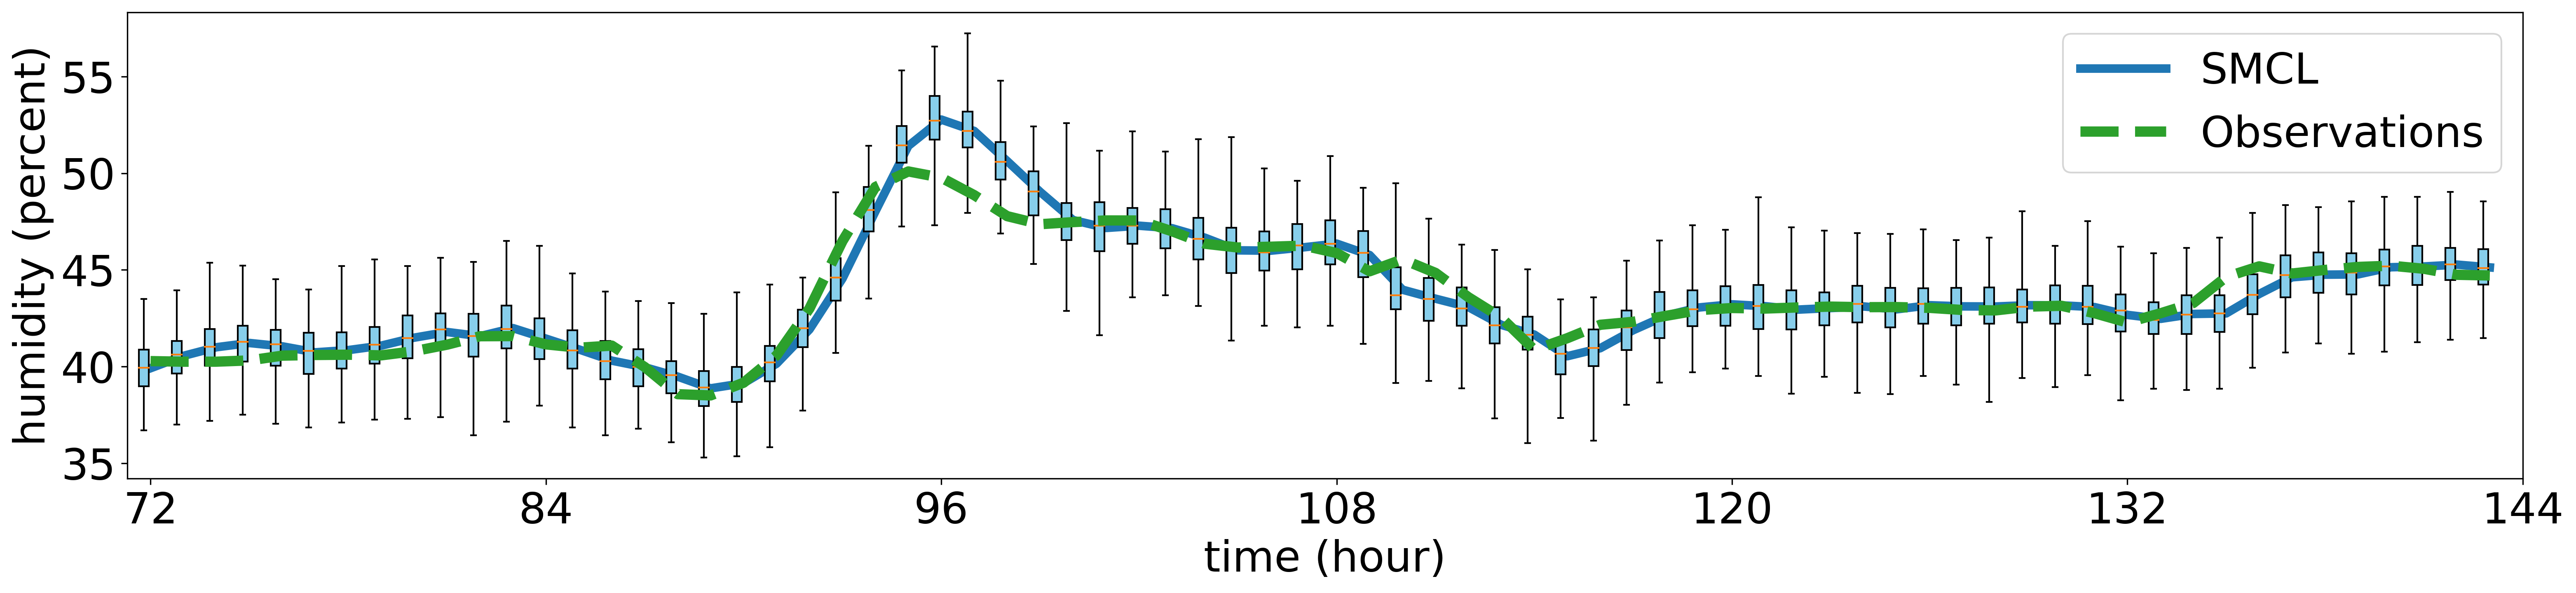
\includegraphics[width=\linewidth]{filter_kp1_hum.png}
	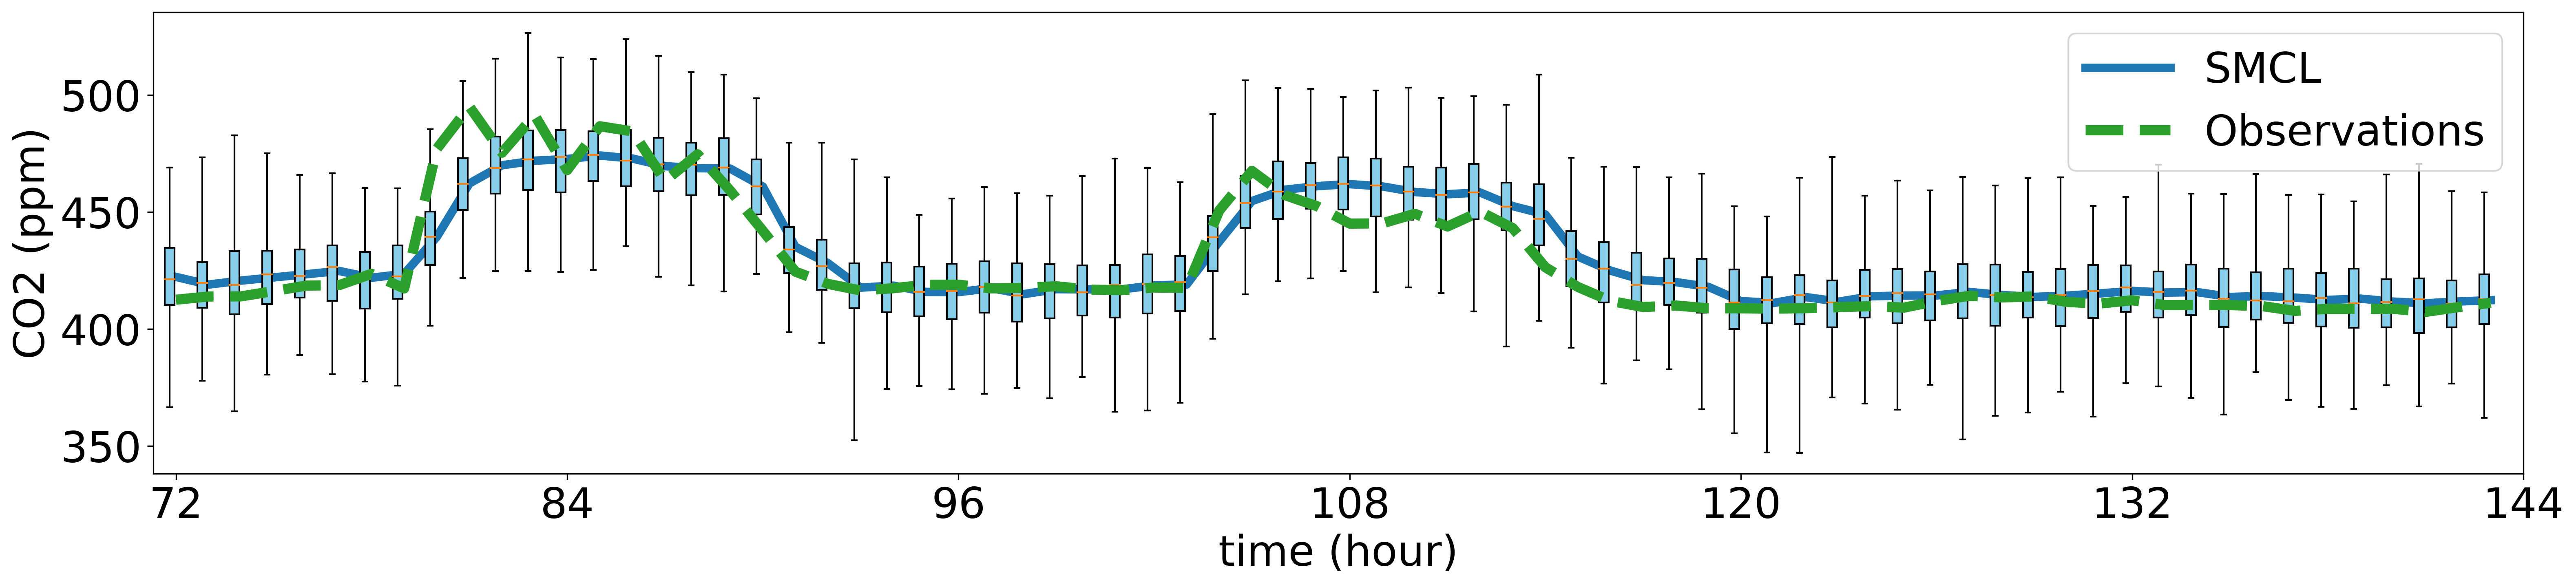
\includegraphics[width=\linewidth]{filter_kp1_co2.png}
	\caption{Prediction of humidity (top) and CO2 (bottom) given previous observations. At each time step, we compute the $N$ predictions associated with current particles, and plot their distributions as boxplot. The box extends from the lower to upper quartile values of the predictions, while the whiskers encloses points below 1.5 time the Interquartile Range.}%
	\label{fig:filter_k+1}
\end{figure*}

\begin{figure*}[htpb]
	\centering
	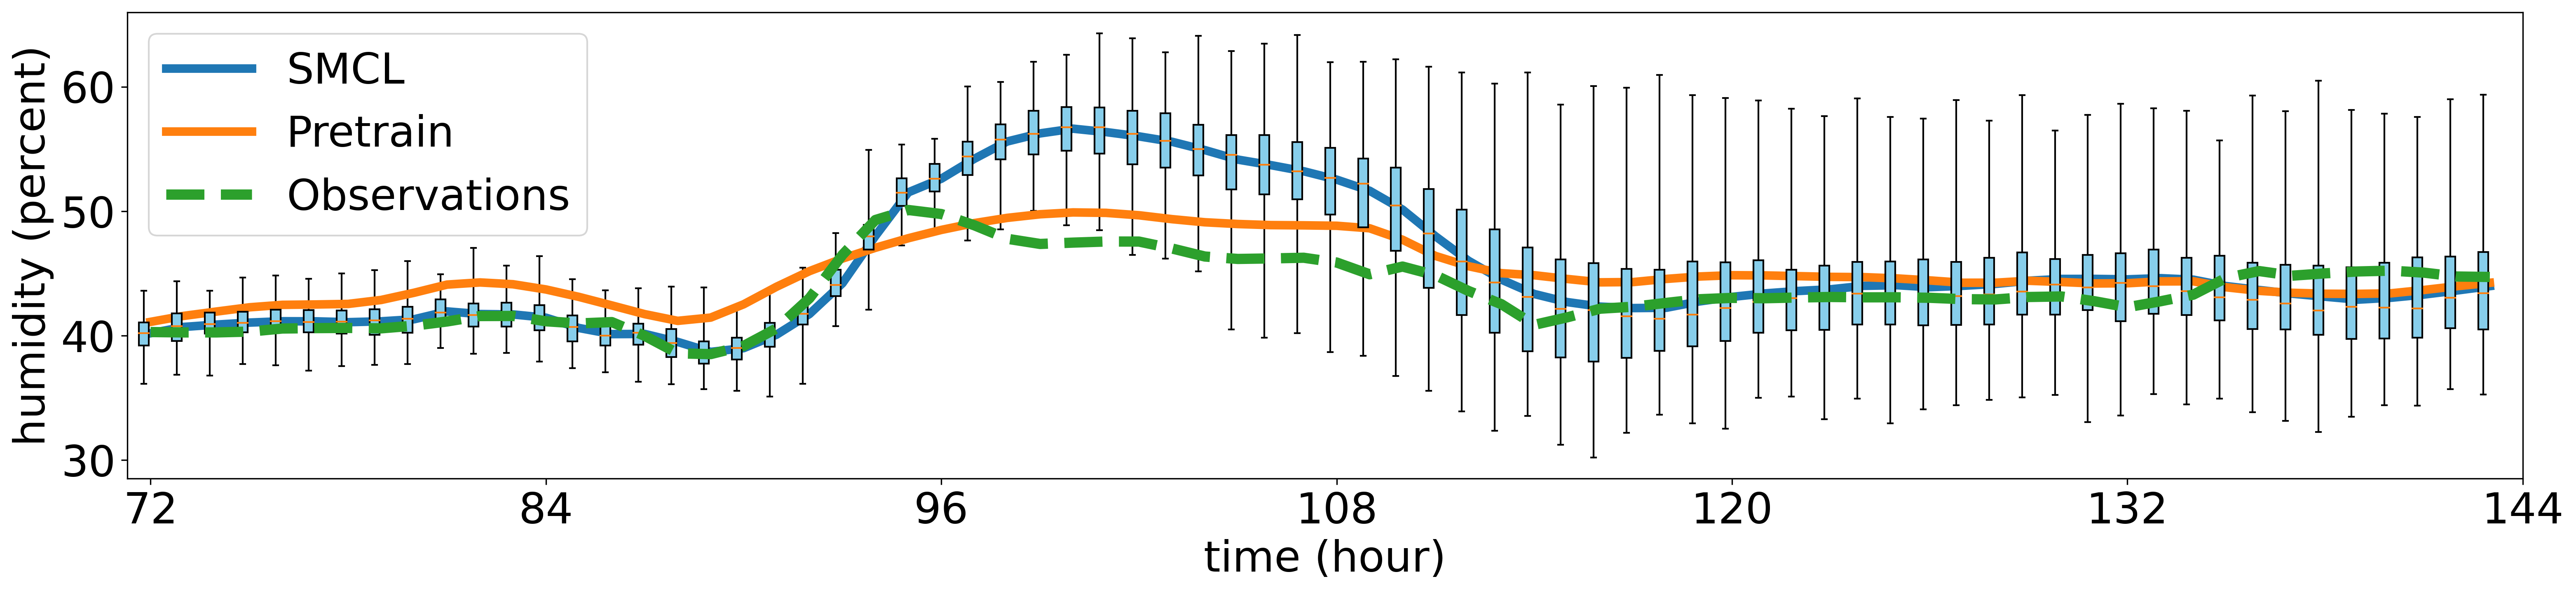
\includegraphics[width=\linewidth]{filter_kp24_hum.png}
	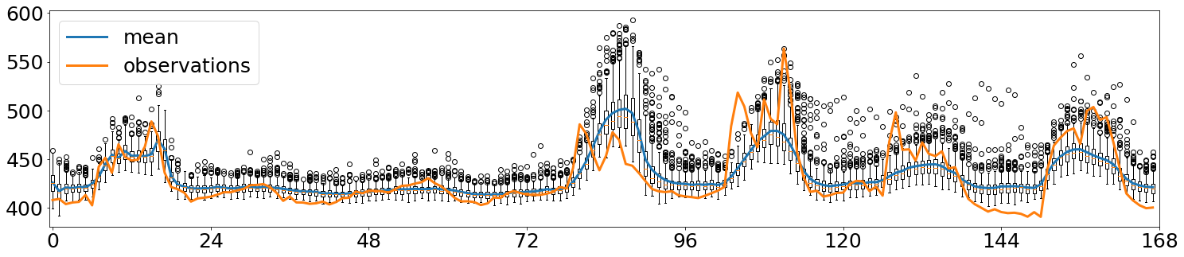
\includegraphics[width=\linewidth]{filter_kp24_co2.png}
	\caption{Prediction of humidity (top) and CO2 (bottom) given observation ($t<72$) and without ($t > 72$). Since re sampling of particles is not longer available, the uncertainty grows.}%
	\label{fig:filter_k+24}
\end{figure*}

\begin{figure*}[htpb]
	\centering
	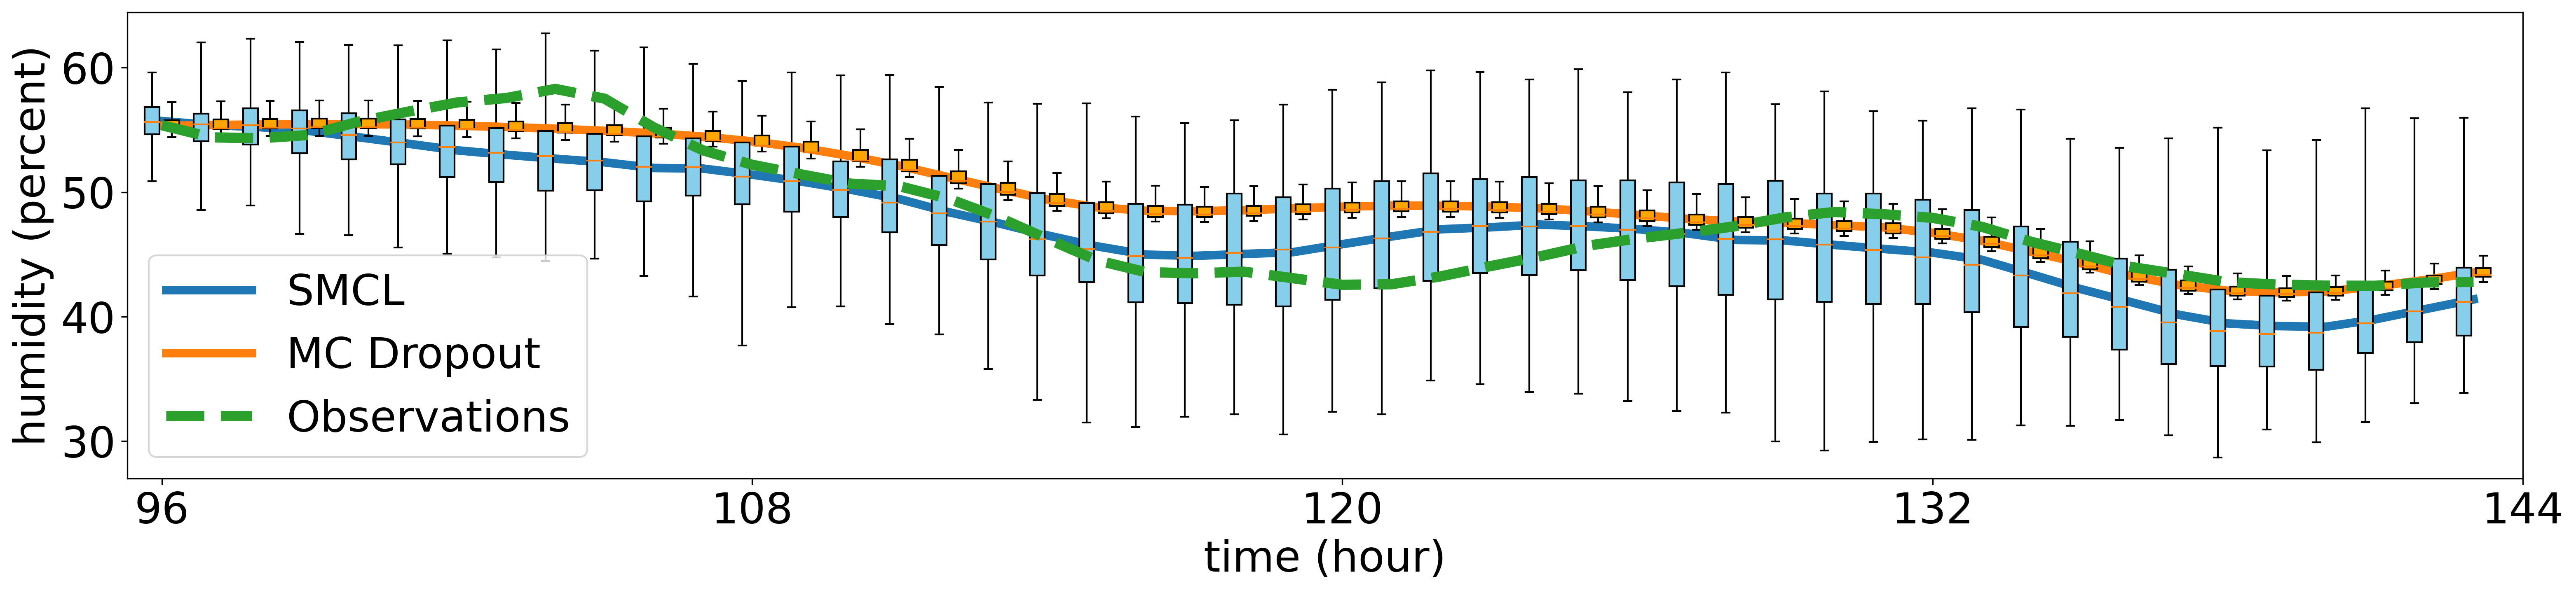
\includegraphics[width=\linewidth]{boxplot_comparison.png}
	\caption{Comparison of confidence intervals and averaged prediction for SMC and MC dropout methods, on a validation sample. For clarity we only display 2 consecutive days, for humidity estimation.}
	\label{fig:boxplot_comparison}
\end{figure*}

\subsection{Evaluations}%
\label{sub:evaluations}

We compare our model to MC Dropout methods on Prediction Interval (PI) metrics introduced in \cite{Pearce2018}.
Given an estimation with lower and upper bound $\hat y_L^{1:T}, \hat y_U^{1:T}$, we compute the Prediction Interval Coverage Probability (PICP) and the Mean Prediction Interval Width as:

\begin{align}
	PICP & = \frac{1}{T} \sum^{T}_{t=1} \mathbb{1}_{[\hat y_L^t, \hat y_U^t]}(y_t) \label{eq:pi_picp} \\
	MPIW & = \frac{1}{T} \sum^{T}_{t=1} \hat y_U^t - \hat y_L^t \label{eq:pi_mpiw}
\end{align}

These estimator are then aggregated on the entire validation set, and their mean and variance are displayed in Table~\ref{tab:ci_comparison}.

\begin{table}[htpb]
	\centering
	\caption{Comparison of PI metrics \ref{eq:pi_picp}, \ref{eq:pi_mpiw} of our model and the LSTM Dropout. Mean values of the estimator on the validation set are displayed, along with their variance.}
	\label{tab:ci_comparison}
	\begin{tabular}{lll}
		\toprule
		             & PICP              & MPIW               \\
		\toprule
		Ours         & $0.99 \pm 0.0002$ & $0.596 \pm 0.0040$ \\
		MC Dropout & $0.23 \pm 0.016$  & $0.195 \pm 0.0011$ \\
		MC Dropout & $0.95 \pm 0.0102$ & $2.330 \pm 0.0535$ \\
		\bottomrule
	\end{tabular}
\end{table}

Evaluations listed in priority order
\begin{enumerate}
	\item Compare confidence interval with MC-dropout model (soit LSTM dropout classique, soit en enlevant la derniere couche)
	\item Compare with ARIMA/classic stat model
	\item Compare MSE (average on particles) with classic finetuning: sample particles for half a week. For the second half, observations are not available at all ; thus we either take the mean of the predictions associated with each particles, or sample from the observation model and take the mean.
	\item Compare linear SMC with kalman filter, sample under the gaussian law, plot boxplot
\end{enumerate}

\section{Conclusion}%
\label{sec:conclusion}

In this paper, we introduced a decoupled architecture for uncertainty estimation on a time series dataset.
Our deep neural network backbone is responsible for extracting high level features, while particle filtering allows modelling recurrent non linear uncertainty.
Our proposed model improves confidence interval quality, compared to MC Dropout methods, while remaining simple and efficient to train, compared to VI alternatives.

We demonstrate the potential behind combining RNN with latent state space models ; more complex architectures, such as GRU or LSTM cells, are left for future works.
Likewise, the poor man's smoother could be replaced by faster and more performant alternatives described above.

Our decoupled architecture enables incorporating uncertainty estimation to an already trained network.
This opens the door to multiple, cheap finetuning of the last layers' parameters and noise estimations, from a global pretraining.
For our application, this could translate in a generic training of the input model on an entire year of weather and building records, followed by season specific finetunings.

% Below is an example of how to insert images. Delete the ``\vspace'' line,
% uncomment the preceding line ``\centerline...'' and replace ``imageX.ps''
% with a suitable PostScript file name.
% -------------------------------------------------------------------------
%\begin{figure}[htb]

%\begin{minipage}[b]{1.0\linewidth}
%  \centering
%  \centerline{\includegraphics[width=8.5cm]{image1}}
%%  \vspace{2.0cm}
%  \centerline{(a) Result 1}\medskip
%\end{minipage}
%%
%\begin{minipage}[b]{.48\linewidth}
%  \centering
%  \centerline{\includegraphics[width=4.0cm]{image3}}
%%  \vspace{1.5cm}
%  \centerline{(b) Results 3}\medskip
%\end{minipage}
%\hfill
%\begin{minipage}[b]{0.48\linewidth}
%  \centering
%  \centerline{\includegraphics[width=4.0cm]{image4}}
%%  \vspace{1.5cm}
%  \centerline{(c) Result 4}\medskip
%\end{minipage}
%%
%\caption{Example of placing a figure with experimental results.}
%\label{fig:res}
%%
%\end{figure}


% To start a new column (but not a new page) and help balance the last-page
% column length use \vfill\pagebreak.
% -------------------------------------------------------------------------
%\vfill
%\pagebreak

% References should be produced using the bibtex program from suitable
% BiBTeX files (here: strings, refs, manuals). The IEEEbib.bst bibliography
% style file from IEEE produces unsorted bibliography list.
% -------------------------------------------------------------------------
\bibliographystyle{IEEEbib}
\bibliography{refs.bib}

\end{document}
